\section{DESARROLLO DEL TRABAJO}

\subsection{Descripción de la solución propuesta}

Se busca desarrollar una aplicación completa que sirva como sistema en gran medida automatizado para obtener una estimación 
de los movimientos realizados por truchas en videos de experimentos \textit{NetTest}. Para realizar esta tarea, se diseñará 
una arquitectura dividida en tres sistemas específicos como se puede ver en la \autoref{fig:ArquitecturaBasicaSolucion}.

\begin{itemize}
    \item Interfaz gráfica de usuario: permitirá al usuario seleccionar el video a analizar, observar los resultados y guardarlos.
    \item Capa de análisis del video: a través de técnicas como el \texttt{Machine Learning} o el análisis de flujo óptico, parametrizará 
    los movimientos de las truchas que aparezcan en el video.
    \item Capa de procesado de datos: obtendrá la caracterización realizada por la capa de análisis y a través de la transformación y 
    procesado de los datos, devolverá los datos que se deban mostrar en la interfaz gráfica. Además realizará la estimación final del número 
    de movimientos por trucha.
\end{itemize}
\begin{figure}[H]
    \centering
    \includegraphics[width=0.9\textwidth]{images/6/IdeaAplicación.png}
    \caption{Arquitectura básica de la solución propuesta}
    \label{fig:ArquitecturaBasicaSolucion}
\end{figure}

El bucle de uso principal consistirá en la selección de un video a procesar, el análisis del mismo, la transformación de los datos resultantes, 
la estimación de los movimientos y la devolución de los datos al usuario a través de la interfaz gráfica.\newline
El usuario podrá elegir verificar los datos o guardar directamente un archivo con los resultados. Realizado esto, el usuario podrá volver a la 
pantalla inicial para seleccionar otro video para continuar con el proceso.

La solución se implementará de manera que se puedan aprovechar al máximo los recursos del sistema, permitiendo una reducción en el tiempo global 
que toma procesar un experimento.

En los siguientes puntos, se explicará el desarrollo que se ha seguido para la implementación de la propuesta, empezando por los componentes internos 
del módulo de obtención de datos, luego su procesado en una arquitectura secuencial y finalmente la implementación en una aplicación completa.

\clearpage
\subsection{Pruebas de concepto: \texttt{OpticalFlow} y \texttt{YOLO}}

El desarrollo del módulo de procesado del video afectaba al tratamiento de datos que se iba a realizar posteriormente, por esto mismo se decidió 
tratarlo como el primer problema a solucionar.

Dentro de este módulo se busca automatizar la obtención de datos y parametrización del movimiento de las truchas dentro del video.

En este sentido se plantearon dos alternativas para su desarrollo usando diferentes tecnologías:

\begin{enumerate}
    \item \textbf{Solución basada en \textit{OpticalFlow}}: La idea general de este método es caracterizar el movimiento de la trucha respecto al 
    fondo de la imagen.\newline
    Si tenemos en cuenta que el análisis por \texttt{OpticalFlow} nos da como resultado una serie de vectores que representan el cambio en los 
    píxeles de la imagen, cabe la posibilidad que con el suficiente preprocesado y estimación de la posición de la trucha, obtener una serie de 
    vectores globales que represen el movimiento de los bordes de la trucha entre fotogramas. La representación de esta idea se puede ver en la \autoref{fig:IdeaOF}.

    \begin{figure}[H]
        \centering
            \begin{subfigure}[b]{\textwidth}
                \centering
                \begin{subfigure}[b]{0.25\textwidth}
                    \centering
                    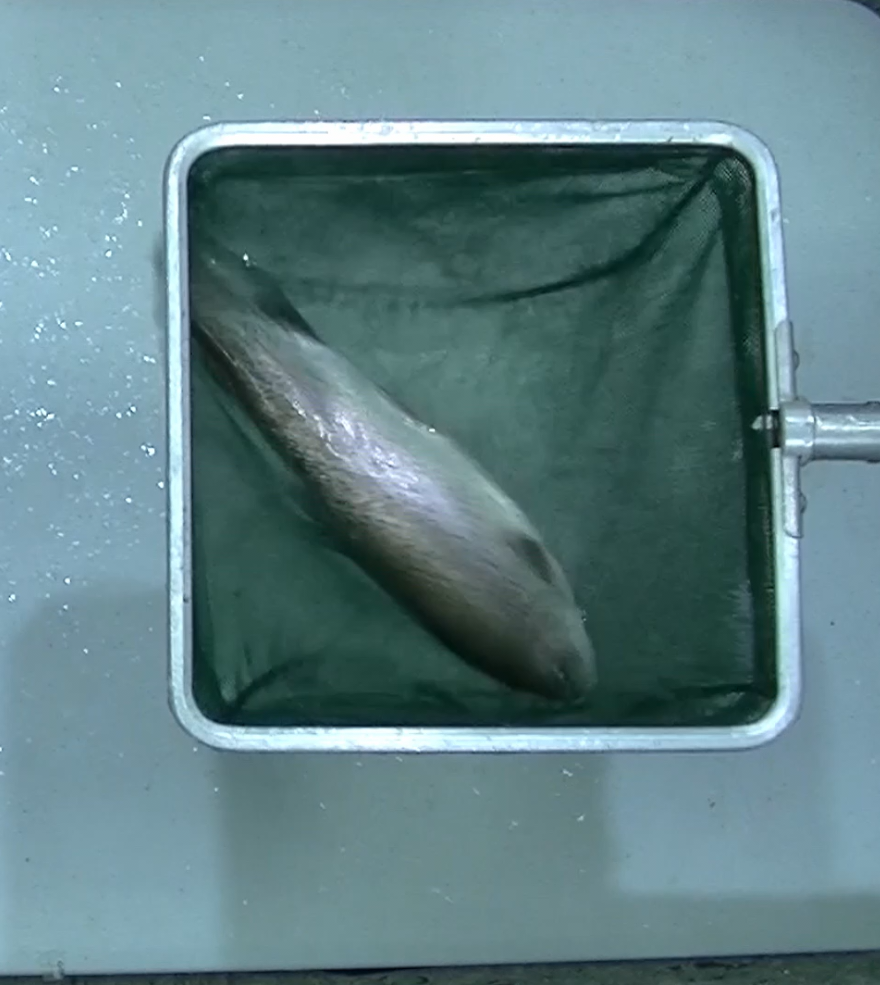
\includegraphics[width=0.8\textwidth]{images/6/SinOptical2.png}
                    \label{fig:SinOptical2}
                \end{subfigure}
                \begin{subfigure}[b]{0.25\textwidth}
                    \centering
                    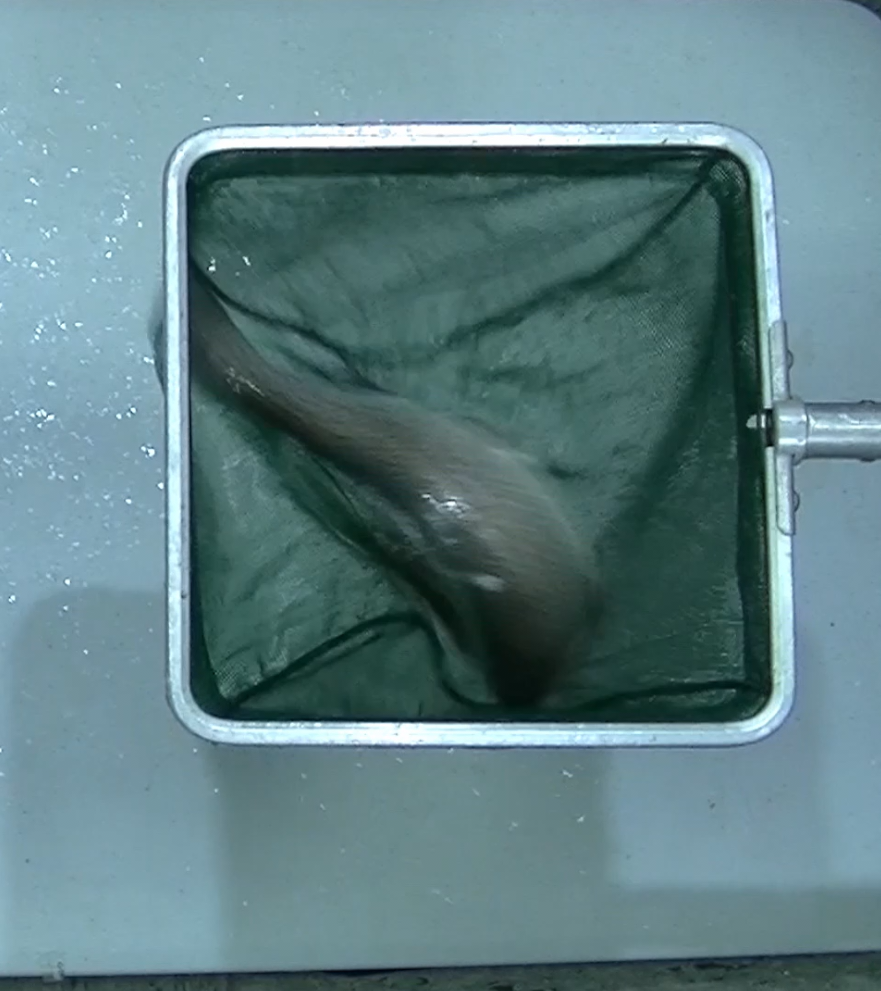
\includegraphics[width=0.8\textwidth]{images/6/SinOptical3.png}
                    \label{fig:SinOptical3}
                \end{subfigure}
                \begin{subfigure}[b]{0.25\textwidth}
                    \centering
                    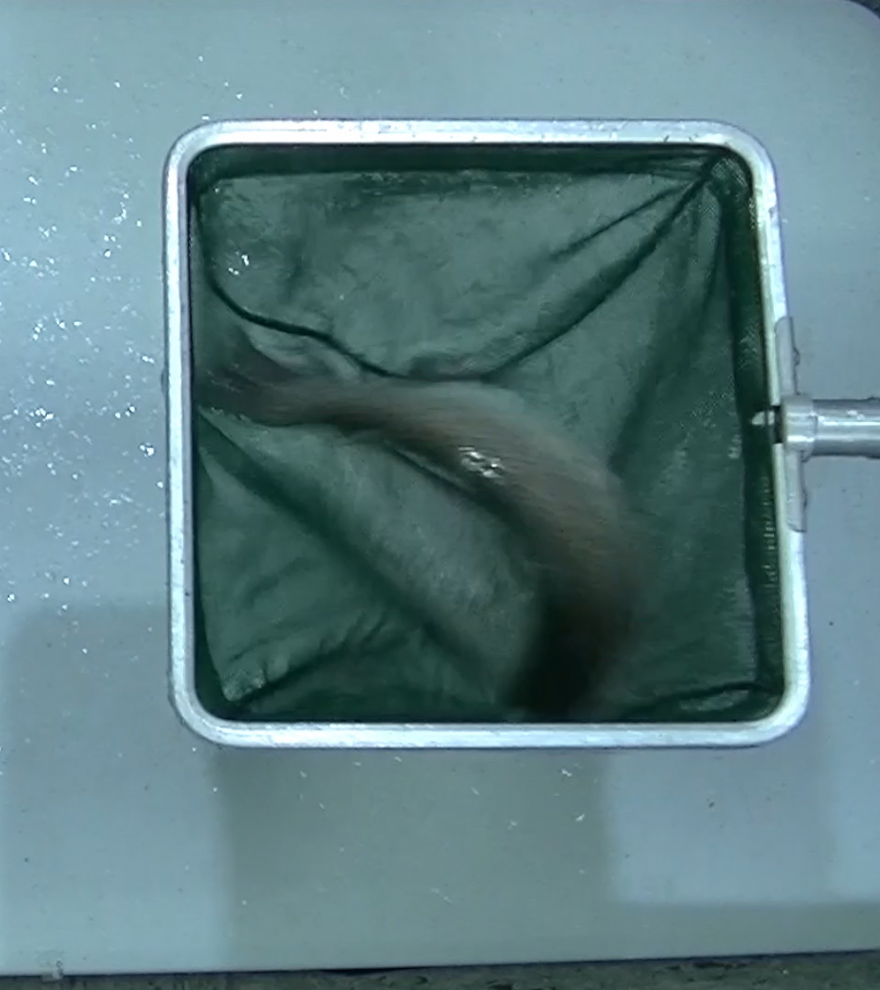
\includegraphics[width=0.78\textwidth]{images/6/SinOptical4.png}
                    \label{fig:SinOptical4}
                \end{subfigure}
                \caption{Fotogramas de entrada}
                \label{fig:FotogramasEntrada}
            \end{subfigure}
            \begin{subfigure}[b]{\textwidth}
                \centering
                \begin{subfigure}[b]{0.25\textwidth}
                    \centering
                    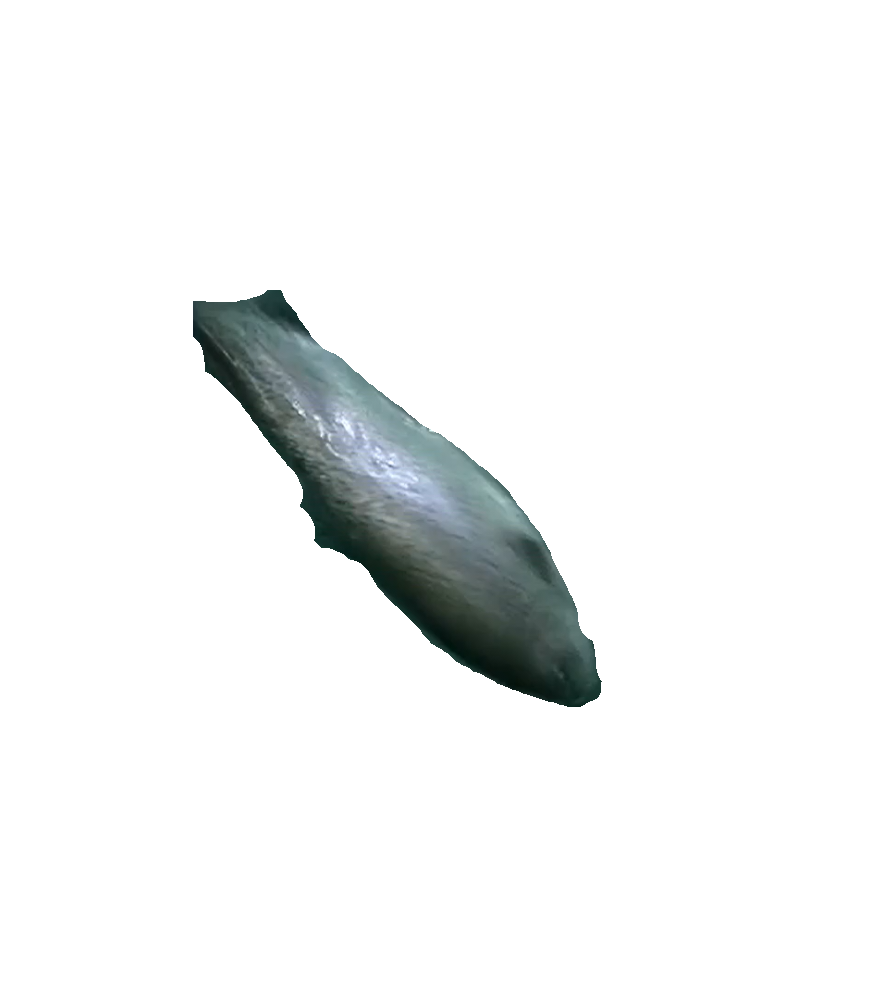
\includegraphics[width=0.8\textwidth]{images/6/Vacio2.png}
                    \label{fig:Vacio2}
                \end{subfigure}
                \begin{subfigure}[b]{0.25\textwidth}
                    \centering
                    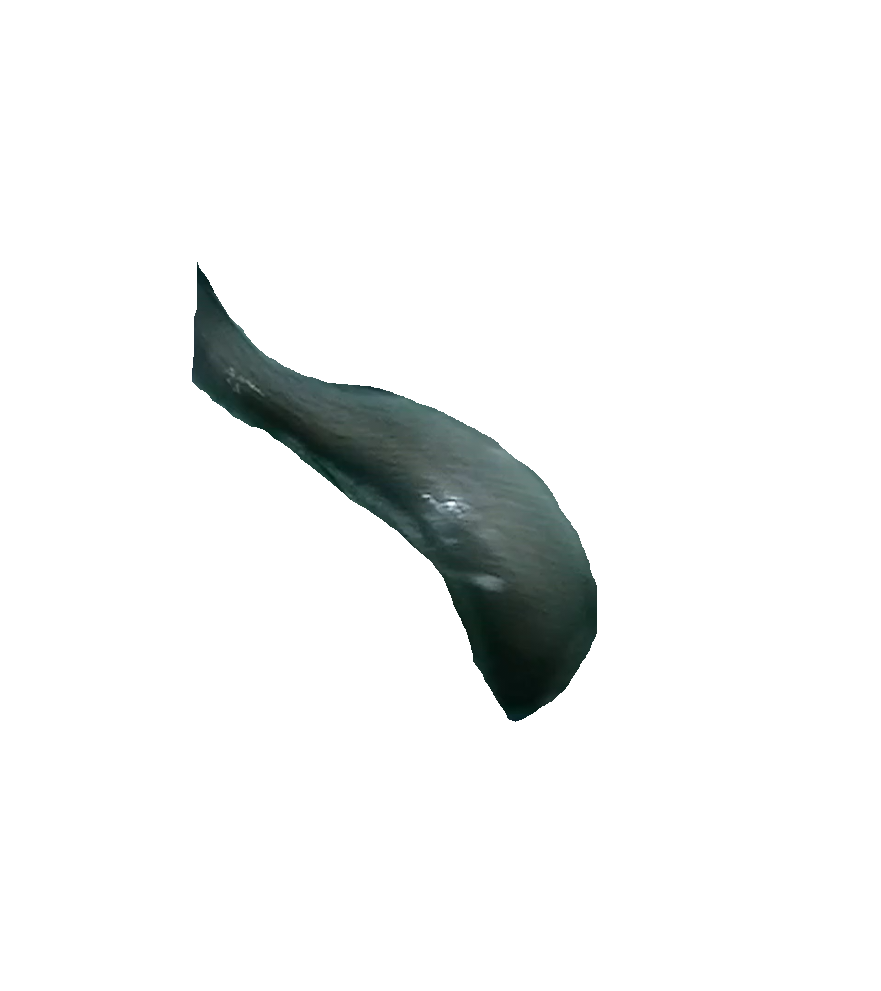
\includegraphics[width=0.8\textwidth]{images/6/Vacio3.png}
                    \label{fig:Vacio3}
                \end{subfigure}
                \begin{subfigure}[b]{0.25\textwidth}
                    \centering
                    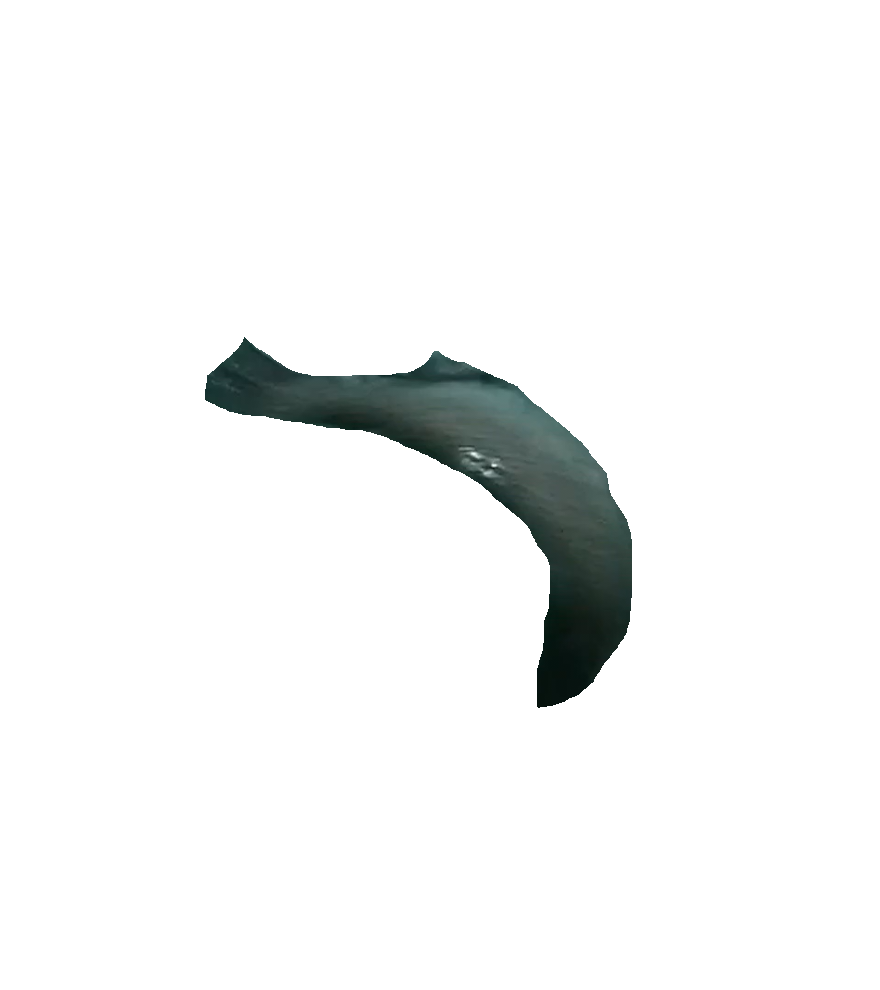
\includegraphics[width=0.8\textwidth]{images/6/Vacio4.png}
                    \label{fig:Vacio4}
                \end{subfigure}
                \caption{Fotogramas con el fondo eliminado}
                \label{fig:FotogramasSilueta}
            \end{subfigure}
            \begin{subfigure}[b]{\textwidth}
                \centering
                \begin{subfigure}[b]{0.25\textwidth}
                    \centering
                    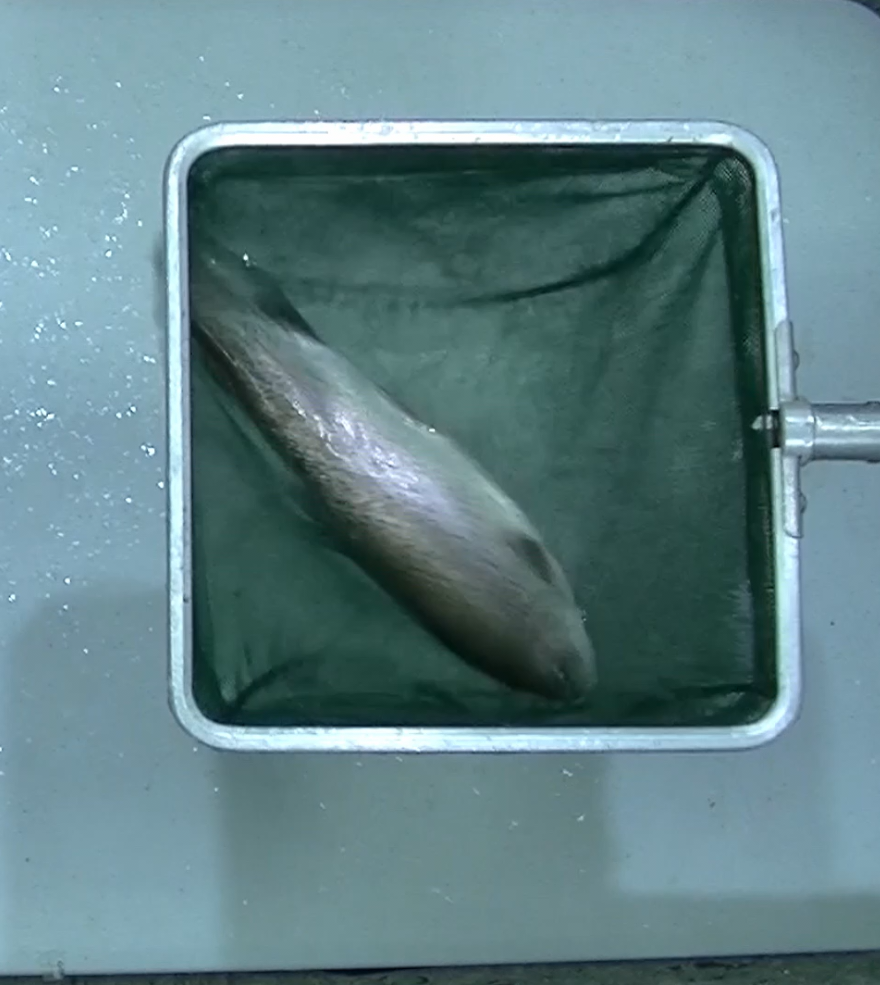
\includegraphics[width=0.8\textwidth]{images/6/SinOptical2.png}
                    \label{fig:Opt2}
                \end{subfigure}
                \begin{subfigure}[b]{0.25\textwidth}
                    \centering
                    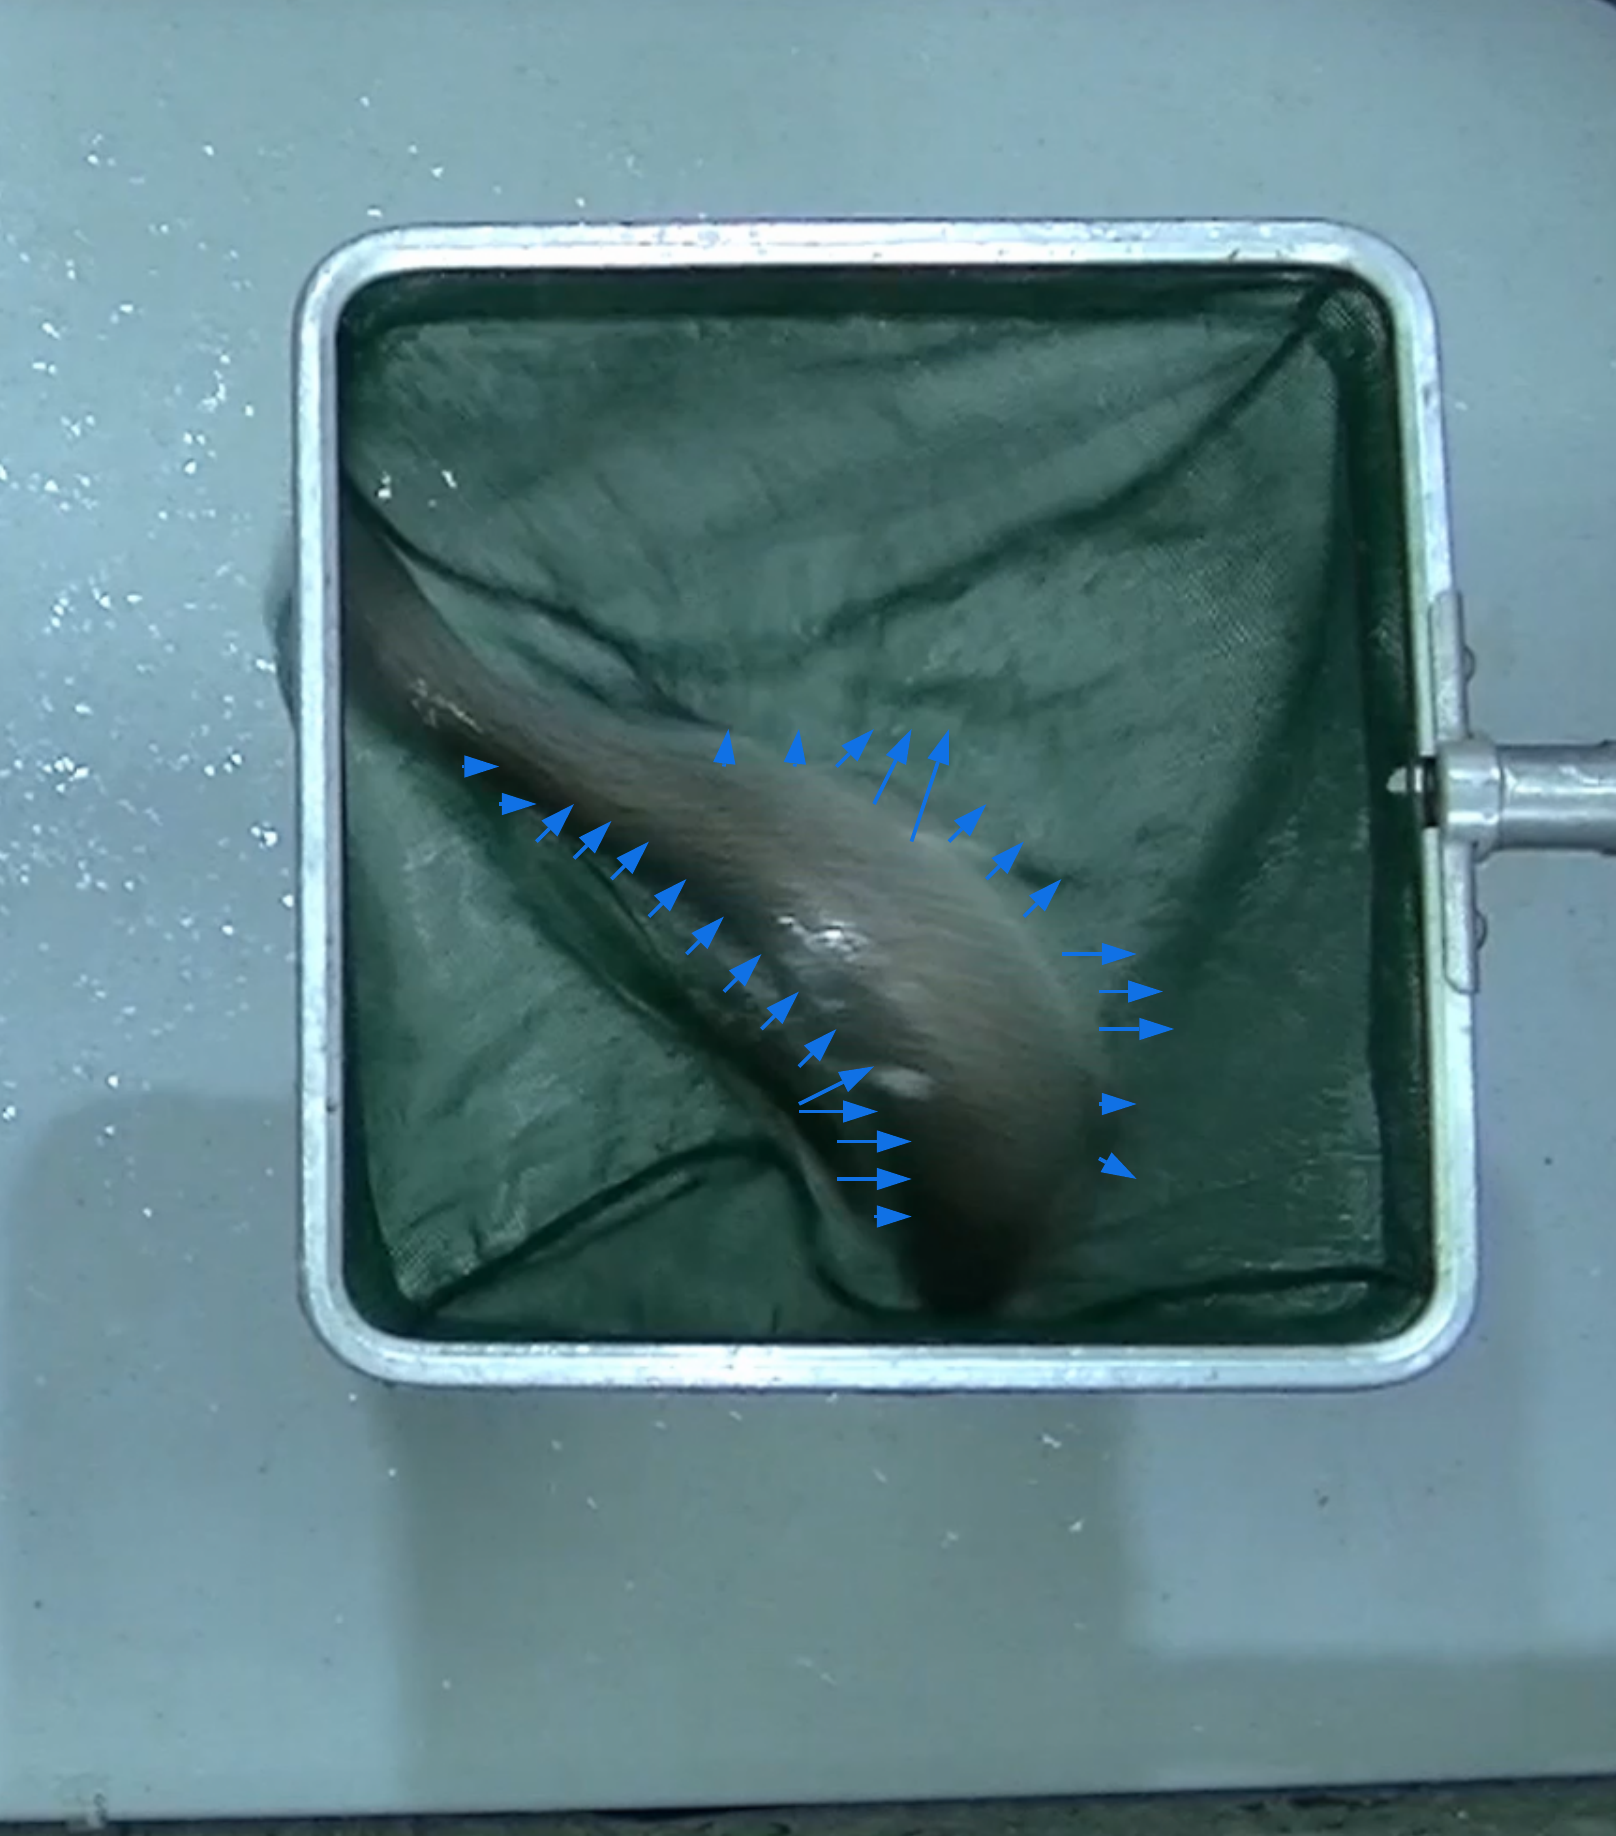
\includegraphics[width=0.8\textwidth]{images/6/ConOptical3.png}
                    \label{fig:Opt3}
                \end{subfigure}
                \begin{subfigure}[b]{0.25\textwidth}
                    \centering
                    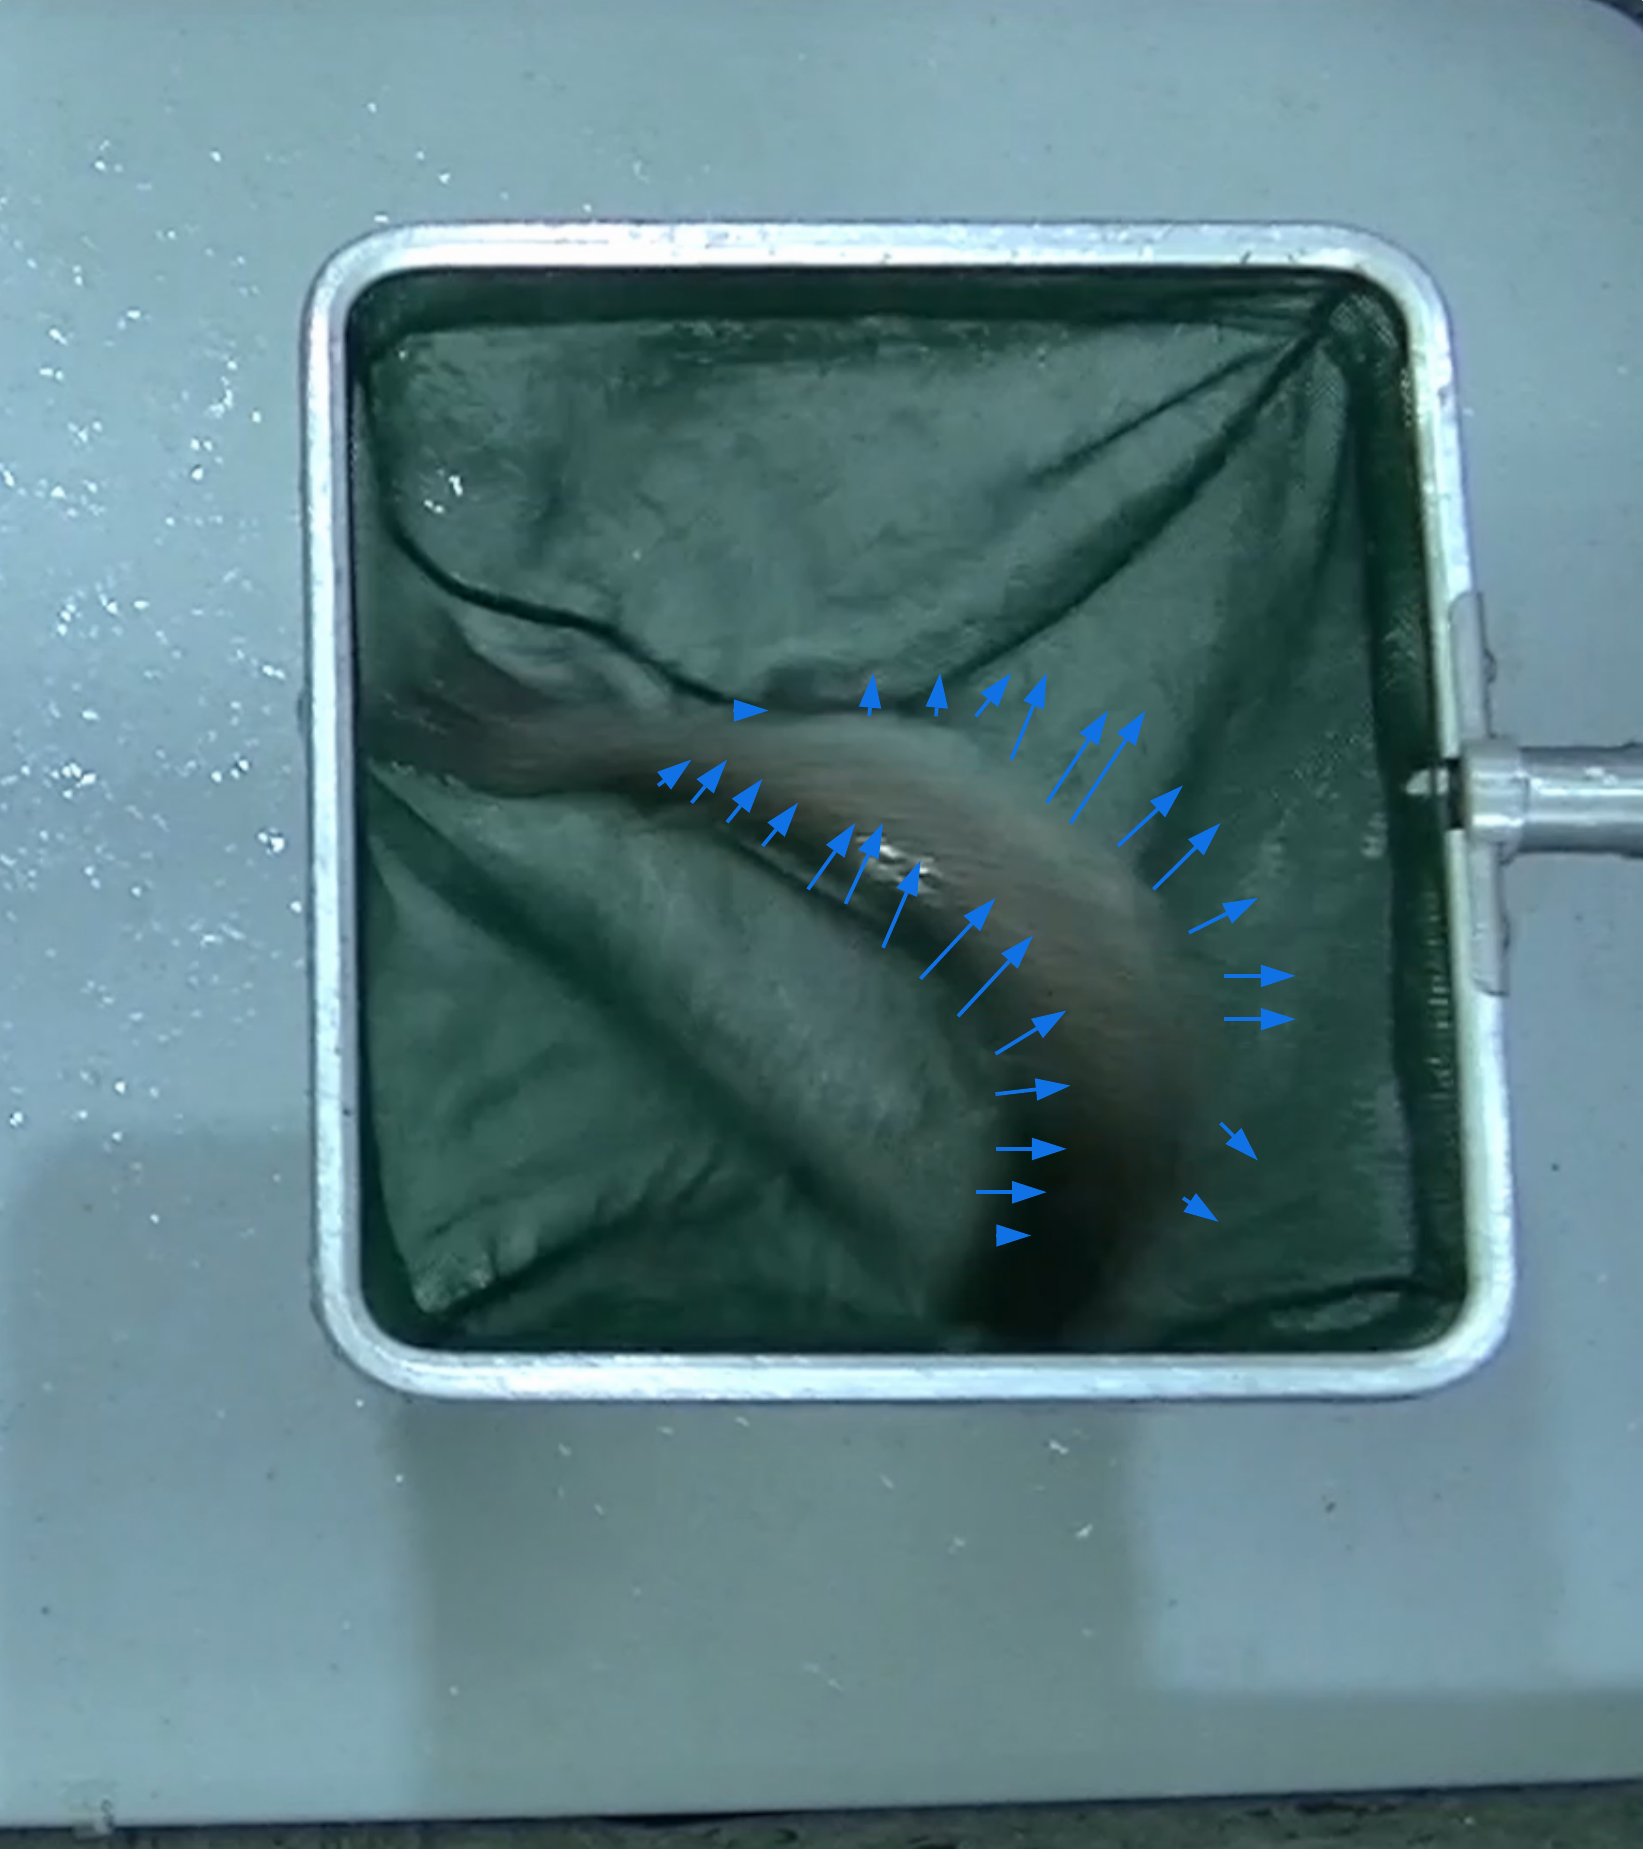
\includegraphics[width=0.8\textwidth]{images/6/ConOptical4.png}
                    \label{fig:Opt4}
                \end{subfigure}
                \caption{Fotogramas con el fondo eliminado}
                \label{fig:FotogramasSalidaOF}
            \end{subfigure}
    \caption{Idea general basada en \texttt{OpticalFlow} para el módulo de procesamiento del video}
    \label{fig:IdeaOF}
    \end{figure}

    Como se puede observar, la idea es obtener un conjunto de vectores en el contorno del pez que nos permitan 
    saber diferentes datos:
    \begin{itemize}
        \item Si se ha movido o no: a través de la suma de todos los vectores y la obtención del 
        módulo del vector global. Si este valor es mayor que cierto umbral, se podría indicar que está sucediendo 
        un movimiento entre los dos fotogramas.
        \item Hacia donde se ha movido: a través del análisis de la dirección del vector global; y si está ocurriendo 
        un movimiento, podemos decir hacia donde está ocurriendo y aportar más información.
    \end{itemize}

    \item \textbf{Solución basada en el uso de \textit{YOLO} como herramienta de análisis}: A través del uso de una \texttt{\acrshort{cnn}} 
    se procesa el video, obteniendo información sobre los objetos detectados como truchas.\newline
    Para realizar esto, hay que definir la tarea que realizaría la red:
    \begin{itemize}
        \item Clasificación: no es útil, ya que no aporta información sobre la posición de los objetos detectados en la imagen.
        \item Segmentación: puede ser útil, pero para entrenar la red en esta tarea, los datos etiquetados deben ser segmentos de la imagen. 
        Esto puede llevar demasiado tiempo y; como se verá más tarde, no es la única tarea que pueda aportar información para la automatización.
        \item Detección: es la más interesante, ya que nos permite conseguir unos tiempos de procesado por imagen muy bajos a la vez que nos da datos 
        relacionados con la posición y el tamaño aproximado de una caja rectangular que envuelva al pez.
    \end{itemize}
    
    Siendo la más viable la tarea de detección, se entrenaría un modelo \texttt{YOLO} para que sea capaz de detectar las truchas. Esto se realizaría 
    conformando un conjunto de datos de imágenes de truchas y sus respectivas etiquetas, que en este caso son dos esquinas de una caja (\texttt{Bounding Box}) que engloba el 
    objeto que se quiere detectar.\newline
    La red neuronal a la hora de realizar la inferencia nos devolvería objetos detectados de esa clase marcados con \texttt{Bounding Boxes} como se puede ver en el ejemplo de la \autoref{fig:IdeaYOLOGeneral}.
    
    A través de estas \texttt{Bounding Boxes}, podemos parametrizar un movimiento como la reducción del área o movimientos de la posición de la \texttt{Bounding Boxes}.

    \begin{figure}[H]
        \centering
        \begin{subfigure}[t]{0.39\textwidth}
            \centering
            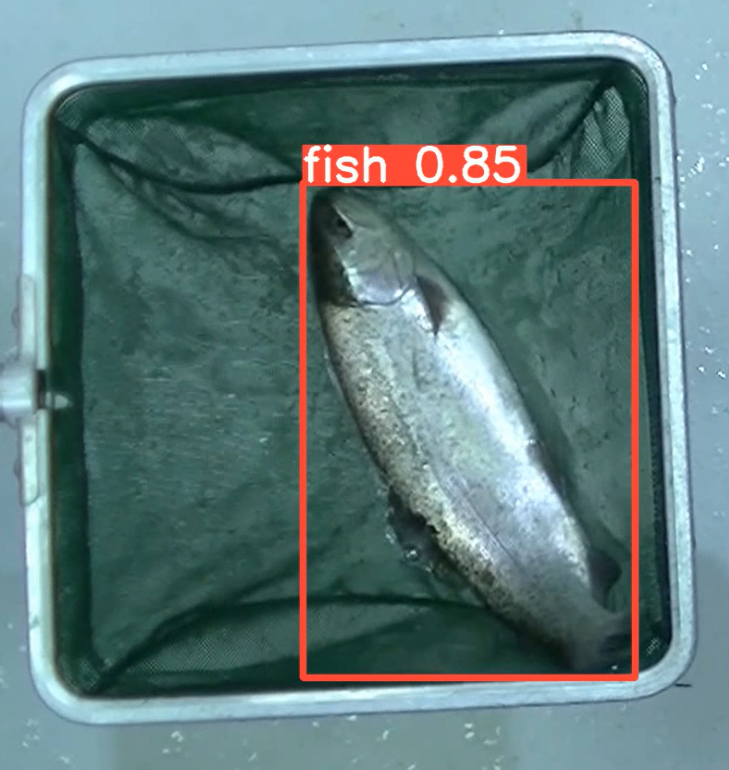
\includegraphics[width=0.8\textwidth]{images/6/EjemploYOLO.png}
            \caption{Imagen procesada por \texttt{YOLO}}
        \end{subfigure}
        \begin{subfigure}[t]{0.59\textwidth}
            \centering
            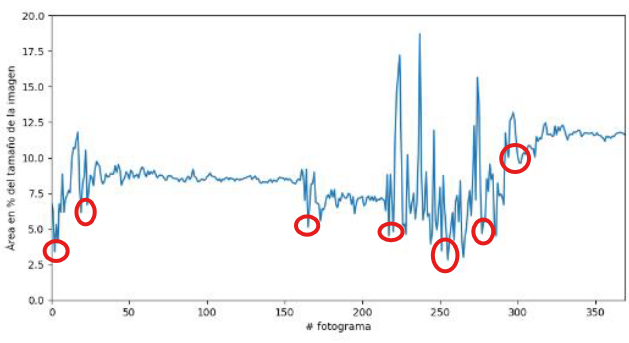
\includegraphics[width=0.99\textwidth]{images/6/YOLOEjemploResultados.png}
            \caption{Idea de estimación de movimiento a través de los resultados de las \texttt{Bounging Boxes}, marcando en rojo los movimientos}
        \end{subfigure}
        \caption{Idea general basada en \texttt{YOLO} para el módulo de procesamiento del video}
        \label{fig:IdeaYOLOGeneral}
    \end{figure}

    Hay que tener en cuenta que sería necesario hacer una validación de los entrenamientos realizados para conseguir cumplir con las necesidades. 
    Esto es debido a que al contrario que el \texttt{OpticalFlow}, las redes neuronales no son deterministas y dependiendo del fotograma sobre el que se realice inferencia, 
    podemos obtener resultados alejados de los esperados.
\end{enumerate}

\vspace{1\baselineskip}
Para decidir cuál método podía dar mejores resultados, se probaron las diferentes tecnologías aplicadas en el video \verb|23_NT_R1_J1_P7_8.mp4|. Este video dura 15 segundos y contiene dos peces, uno a 
la izquierda y otro a la derecha.

\clearpage
\subsubsection{Pruebas de concepto con \texttt{OpticalFlow}}

Para realizar las pruebas se utilizó el entorno de \texttt{MATLAB} en la versión \texttt{2023B}. En esta aplicación se disponen de 2 funciones principales 
que implementan análisis de flujo óptico: 
\begin{itemize}
    \item Método de Horn-Schunck: método de análisis denso (aplicado para todos los píxeles de la imagen).
    \item Método de Lucas-Kanade: método de análisis local (aplicado a áreas de píxeles que se asumen que tienen el mismo movimiento).
\end{itemize}

Ambas pruebas demostraron que los videos con los que se estaba trabajando tenían una tasa de fotogramas demasiado baja para la cantidad de movimiento que podía ocurrir entre fotogramas. 
Esto se puede observar en el flujo óptico percibido cuando suceden cambios bruscos del pez como en la \autoref{fig:HSOpticalFlow} para el método Horn-Schunck y en la \autoref{fig:LKOpticalFlow} 
para el método Lucas-Kanade.

\begin{figure}[H]
    \centering
    \begin{subfigure}[b]{0.49\textwidth}
        \centering
        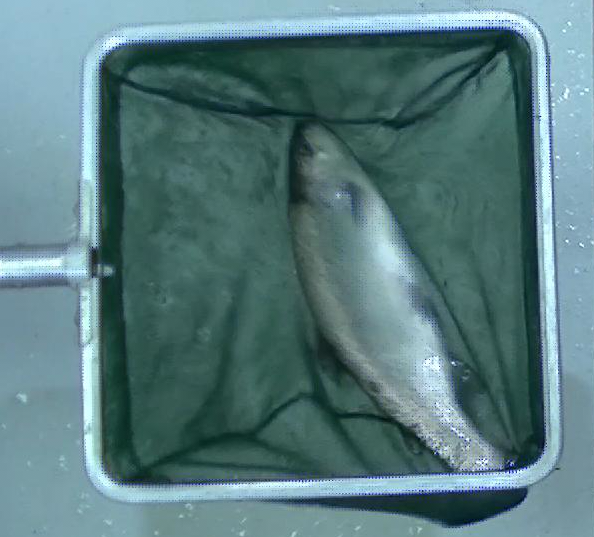
\includegraphics[width=0.95\textwidth]{images/6/6.2.1/HSIzquierda1.png}
    \end{subfigure}
    \begin{subfigure}[b]{0.49\textwidth}
        \centering
        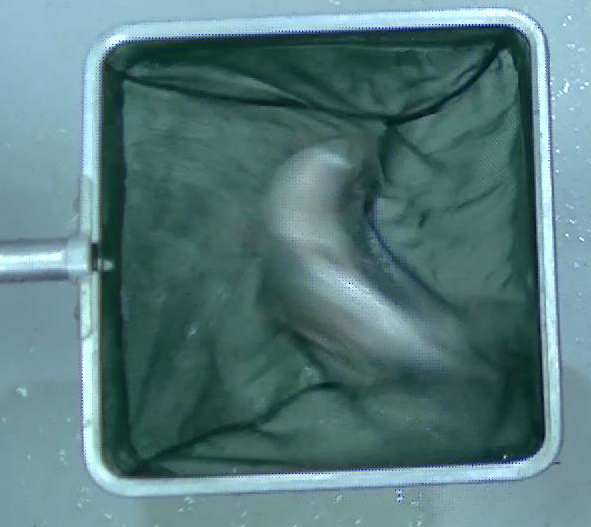
\includegraphics[width=0.95\textwidth]{images/6/6.2.1/HSIzquierda2.png}
    \end{subfigure}
    \caption{Flujo óptico detectado entre dos fotogramas por el método Horn-Schunck en los videos del \textit{NetText}}
    \label{fig:HSOpticalFlow}
\end{figure}

\begin{figure}[H]
    \centering
    \begin{subfigure}[b]{0.45\textwidth}
        \centering
        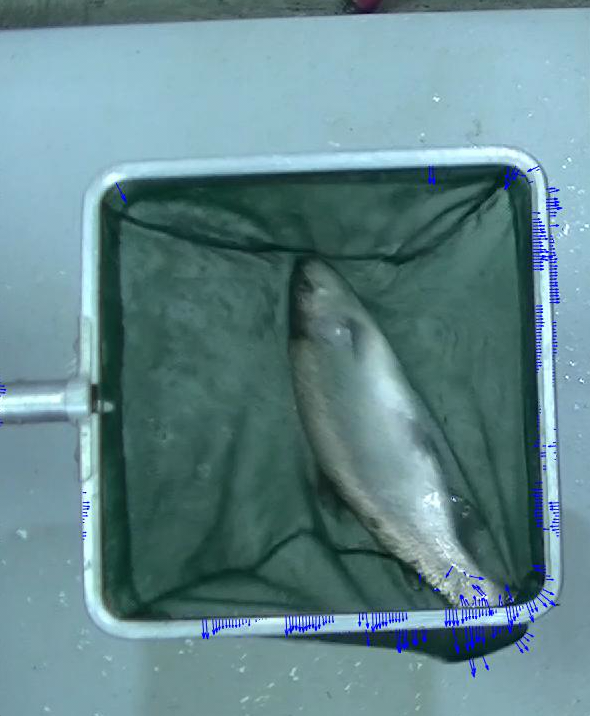
\includegraphics[width=0.8\textwidth]{images/6/6.2.1/LKIzquierda1.png}
    \end{subfigure}
    \begin{subfigure}[b]{0.45\textwidth}
        \centering
        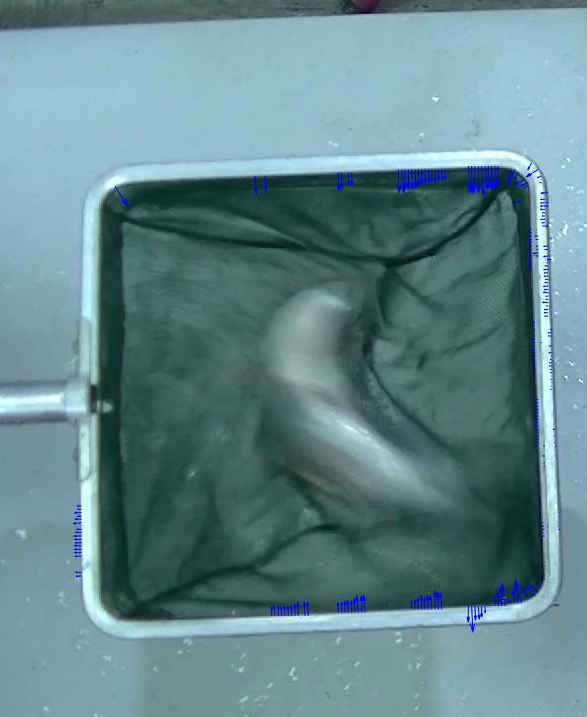
\includegraphics[width=0.8\textwidth]{images/6/6.2.1/LKIzquierda2.png}
    \end{subfigure}
    \caption{Flujo óptico detectado entre dos fotogramas por el método Lucas-Kanade en los videos del \textit{NetText}}
    \label{fig:LKOpticalFlow}
\end{figure}

El principal problema del método Horn-Schunck es que se ve muy afectado por el ruido, en el caso de este experimento, ese ruido aparece por el poco \texttt{bitrate} que tiene el video 
en comparación con la velocidad de movimiento que tienen las truchas. Aparte de esto, es un método computacionalmente muy costoso. en el caso de este video de 15 segundos tardó cerca de 10 
minutos en realizar el análisis completo del flujo óptico, lo cual incumple el requisito 18.

Vemos cierta mejoría usando el método de Lucas-Kanade, pero al realizar el análisis de forma local en zonas con similitudes, en cuanto la trucha hace un movimiento, el análisis deja de funcionar 
sobre la parte de la imagen en la que se sitúa la trucha. Aún siendo bastante rápido (sin llegar a ser tiempo real), esta situación elimina la posibilidad de utilizar este método para la 
parametrización del movimiento de la trucha.

En ambos métodos se ha comprobado que mejorarían los resultados aplicando umbralizaciones a la imagen. También sería necesario un preprocesado para delimitar la sección de 
imagen sobre la que es de interés realizar el análisis de flujo óptico (la zona de la red que contiene la trucha). Aún con lo comentado anteriormente, el único método que puede aportar algún 
tipo de información de manera consistente para todo el video es el método de Horn-Schunck.

\subsubsection{Pruebas de concepto con \texttt{YOLO}}

Para realizar esta prueba, creo un conjunto de datos con el que entrenar a través de fotogramas del video \verb|23_NT_R1_J1_P1_2.mp4|. Esto se realizó a través de la herramienta \texttt{\acrfullr{cvat}}.\newline
Esta herramienta de código abierto\cite{cvat.aicorporationComputerVisionAnnotation2023} es mantenida por los creadores de la librería \texttt{OpenCV}. Dispone de una versión online limitada al número de 
archivos que se pueden subir a \texttt{500 MB} y en otros aspectos, pero también dispone de una versión desplegable por \texttt{Docker}. Uno de sus puntos fuertes y el motivo de su uso en este trabajo es 
la compatibilidad con muchos formatos de exportación de etiquetas.

Como parte de este proyecto y como sistema que sirviese de soporte para guardar todos los conjuntos de datos necesarios, se desplegó como contenedor en el servidor \acrfullr{nas} del \acrfullr{gamma}.

Con esta aplicación se realizó el etiquetado de 24 imágenes para realizar un primer entrenamiento, el conjunto de datos se dividió de la siguiente manera:
\begin{itemize}
    \item 16 imágenes para el conjunto de entrenamiento.
    \item 4 imágenes para el conjunto de validación.
    \item 4 imágenes para el conjunto de pruebas
\end{itemize}

Posteriormente se realizó el entrenamiento de la red neuronal \texttt{YOLOv8} versión \texttt{nano}, que es la más pequeña y rápida de entrenar. Los detalles en profundidad de resultados de este 
entrenamiento se pueden observar en el \hyperref[train:1]{anexo B}. \newline
Se consiguió unos buenos resultados y al inferir sobre el video \verb|23_NT_R1_J1_P7_8.mp4|, se observó que el seguimiento de la trucha se conseguía incluso en situaciones críticas donde la trucha realizaba 
el movimiento como en la \autoref{fig:YOLOTrain1Bien}. Sin embargo, situaciones como las de la \autoref{fig:YOLOTrain1Mal},en donde la trucha tenía formas suficientemente extrañas o se ocultaba detrás del marco de la red resaltaron la falta de entrenamiento y la 
necesidad de expandir el conjunto de datos.
\begin{figure}[H]
    \centering
    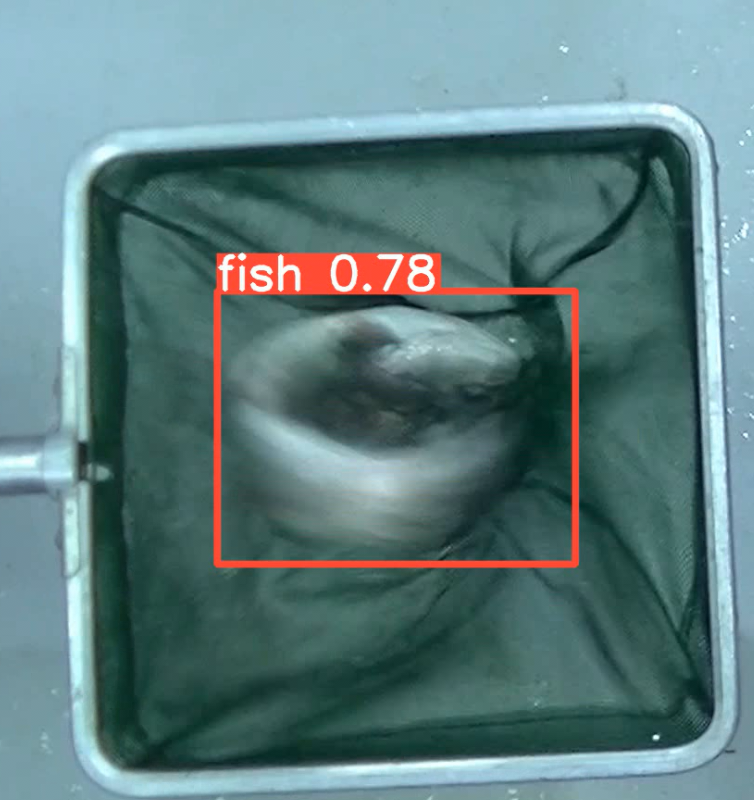
\includegraphics[width=0.3\textwidth]{images/6/6.2.2/DeteccionTrain1.png}
    \caption{Correcta detección en la prueba de concepto de \texttt{YOLO} en situaciones de movimiento}
    \label{fig:YOLOTrain1Bien}
\end{figure}

\begin{figure}[H]
    \centering
    \begin{subfigure}[b]{0.4\textwidth}
        \centering
        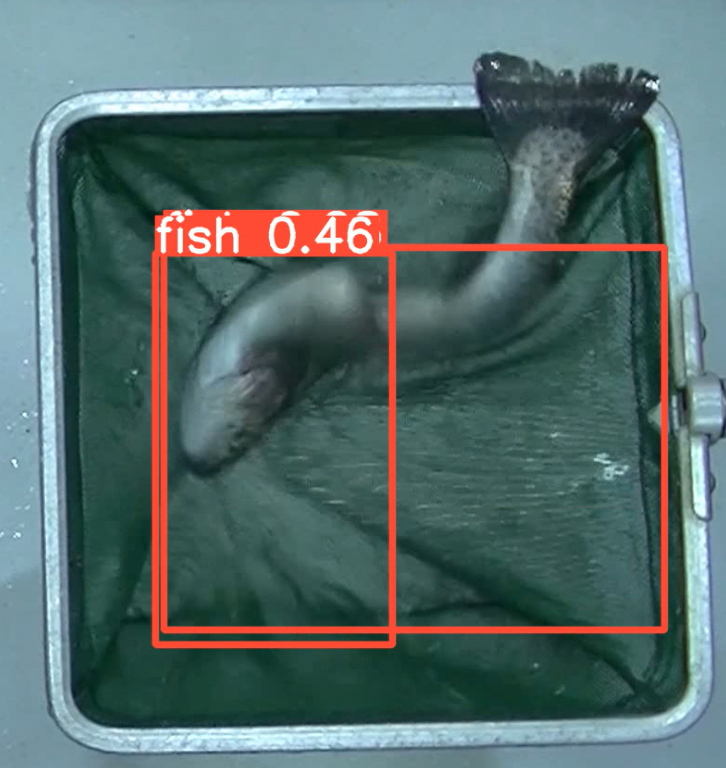
\includegraphics[width=0.7\textwidth]{images/6/6.2.2/DeteccionRaraTrain1.png}
        \caption{Detección de poca confianza y de baja calidad en el primer entrenamiento}
    \end{subfigure}
    \begin{subfigure}[b]{0.5\textwidth}
        \centering
        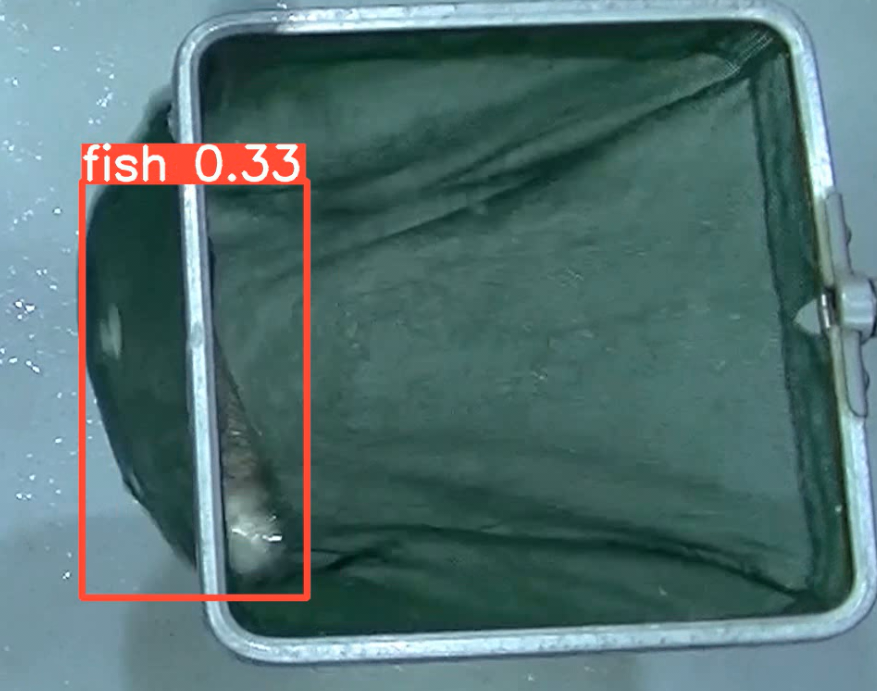
\includegraphics[width=0.7\textwidth]{images/6/6.2.2/PocaConfianzaTrain1.png}
        \caption{Detección de poca confianza por ocultación de la trucha}
    \end{subfigure}
    \caption{Situaciones negativas en la prueba de concepto de \texttt{YOLO}}
    \label{fig:YOLOTrain1Mal}
\end{figure}

\vspace{3\baselineskip}

Hay que hablar del entrenamiento, conjunto de datos usado, verificación de resultados, tiempo de procesado, viabilidad de solución, estimación de movimiento a través de las áreas de las bounding 
boxes.

Finalmente hablar de los resultados publicados en el congreso de Álvaro y su respectiva cita.

\clearpage
\subsection{Pruebas de desarrollo: sistema \texttt{StandAlone} con \texttt{YOLO}}



\clearpage
\subsection{Desarrollo de aplicación completa}